\section{二氧化碳的制取和性质}\label{sec:xssy-sy5}

\begin{shiyanmudi}
    1. 学会二氧化碳的实验室制法和用向上排空气法收集气体; 2. 试验二氧化碳的性质。
\end{shiyanmudi}


\begin{shiyanyongpin}
    烧杯、集气瓶、量筒、平底烧瓶、导管、橡皮管、单孔橡皮塞、铁架、试管、试管夹、玻璃片、酒精灯、蜡烛、木条。

    碳酸钙、稀盐酸($1:2$)、石灰水、石蕊试液、蒸馏水。
\end{shiyanyongpin}


\begin{shiyanbuzhou}
    1. 制取二氧化碳

    (1) 按照图 \ref{fig:xssy-23} 那样把装置连接好。检查这个装置的气密性。

    \begin{figure}[htbp]
        \centering
        \begin{minipage}[b]{7cm}
            \centering
            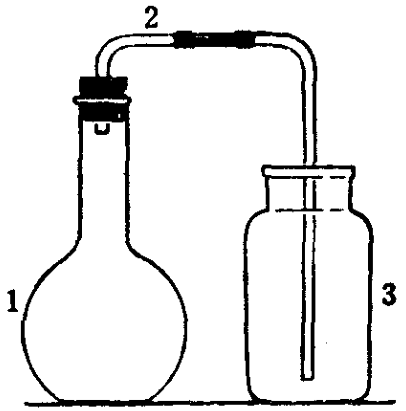
\includegraphics[width=5cm]{../pic/czhx1-xssy-23}
            \caption{制取二氧化碳的装置}\label{fig:xssy-23}
        \end{minipage}
        \qquad
        \begin{minipage}[b]{7cm}
            \centering
            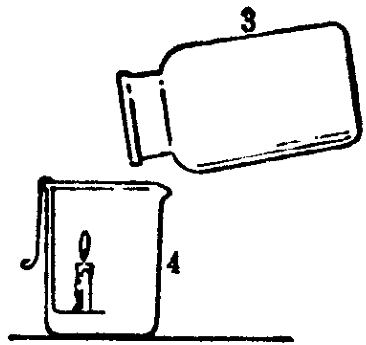
\includegraphics[width=5cm]{../pic/czhx1-xssy-24}
            \caption{把二氧化碳倒入燃着蜡烛的烧杯里}\label{fig:xssy-24}
        \end{minipage}
    \end{figure}

    (2) 在平底烧瓶 1 里放入几小块碳酸钙(想一想应该怎么放)。然后小心地注入稀盐酸 15 毫升。
    立即用带有导管 2 的橡皮塞塞住瓶口,观察烧瓶里发生的现象以及反应中产生气体的颜色。
    过一会儿,可用燃着的木条检查集气瓶 3 里是不是已集满二氧化碳(检查时,木条应放在瓶口还是伸入瓶内)。
    用玻璃片盖住已集满二氧化碳的集气瓶。记录实验现象,并写出有关反应的化学方程式。

    2. 试验二氧化碳的性质

    (1) 把一支短蜡烛固定在烧杯 4 的铁架上,用火点着。
    拿起集满二氧化碳的集气瓶 3,象倒水一样,把二氧化碳倒入烧杯 4 里(图 \ref{fig:xssy-24})。
    观察有什么现象发生。这个实验证明二氧化碳具有什么性质?

    (2) 在一个试管里注入少量澄清的石灰水,通入二氧化碳,发生什么现象?
    继续通入二氧化碳,又有什么现象发生?如果试管里的液体变得澄清,用试管夹夹住试管进行加热,又有什么现象发生?
    解释这一系列变化的原因,并写出这些反应的化学方程式。

    如果从实验步骤 1 制得的二氧化碳的量,不足以供继续实验用,可以把烧瓶 1 里的残留物倒掉,
    另加入几小块碳酸钙和 10—15 毫升稀盐酸,重新制取二氧化碳。

    (3) 在一个试管里加入 2 毫升蒸馏水,滴入 1—2 滴石蕊试液,观察溶液的颜色。
    通入二氧化碳,再观察溶液的颜色有没有变化? 为什么?
\end{shiyanbuzhou}


\begin{wentihetaolun}
    1. 通过以上实验,证明二氧化碳有哪些物理性质和化学性质?

    2. 用排水法和排空气法(又分向上和向下两种)收集气体,分别根据气体的什么性质?
    如要收集氧气、氢气和二氧化碳气体,可分别用什么方法?

    3. 有四瓶无色气体,分别是空气、氢气、氧气和二氧化碳。怎样鉴别它们?叙述操作过程和可能观察到的现象。

    4. 怎样证明鸡蛋壳和锅炉水垢里的主要成分是碳酸钙?
\end{wentihetaolun}

